\documentclass[aspectratio=169]{beamer}
\usetheme{Madrid}
\usepackage{booktabs}
\usepackage{graphicx}
\usepackage{array}

\title{Branch Specialization Checkpoint}
\subtitle{Explicit Branch Isolation}
\author{Branch Specialization Project}
\date{2026-05-22}

\begin{document}

\begin{frame}
  \titlepage
  \vspace{-0.5em}
  \begin{center}
    Checkpoint reason: explicit routing separates specialization from modularity.
  \end{center}
\end{frame}

\begin{frame}{Question}
  Previous toy results showed:
  \begin{itemize}
    \item head-dimension heterogeneity can stabilize functional specialization;
    \item adding a second high-capacity head does not force modular role separation.
  \end{itemize}

  \vspace{0.8em}
  This checkpoint asks:

  \begin{quote}
    Is explicit branch routing needed to turn specialization into functional modularity?
  \end{quote}
\end{frame}

\begin{frame}{Setup}
  Same local-vs-induction competition task:
  \begin{itemize}
    \item local copy: \texttt{[x, SEP, x]};
    \item induction continuation: \texttt{[y1,...,y16,y1,...,y16]};
    \item local weight 0.25, induction weight 1.0;
    \item five seeds per config.
  \end{itemize}

  \vspace{0.6em}
  Branch variants:
  \begin{itemize}
    \item \texttt{branch\_sum}: two separate branch towers, both active everywhere.
    \item \texttt{oracle\_route}: local positions use branch 0; induction positions use branch 1.
  \end{itemize}
\end{frame}

\begin{frame}{Main Evidence}
  \begin{center}
  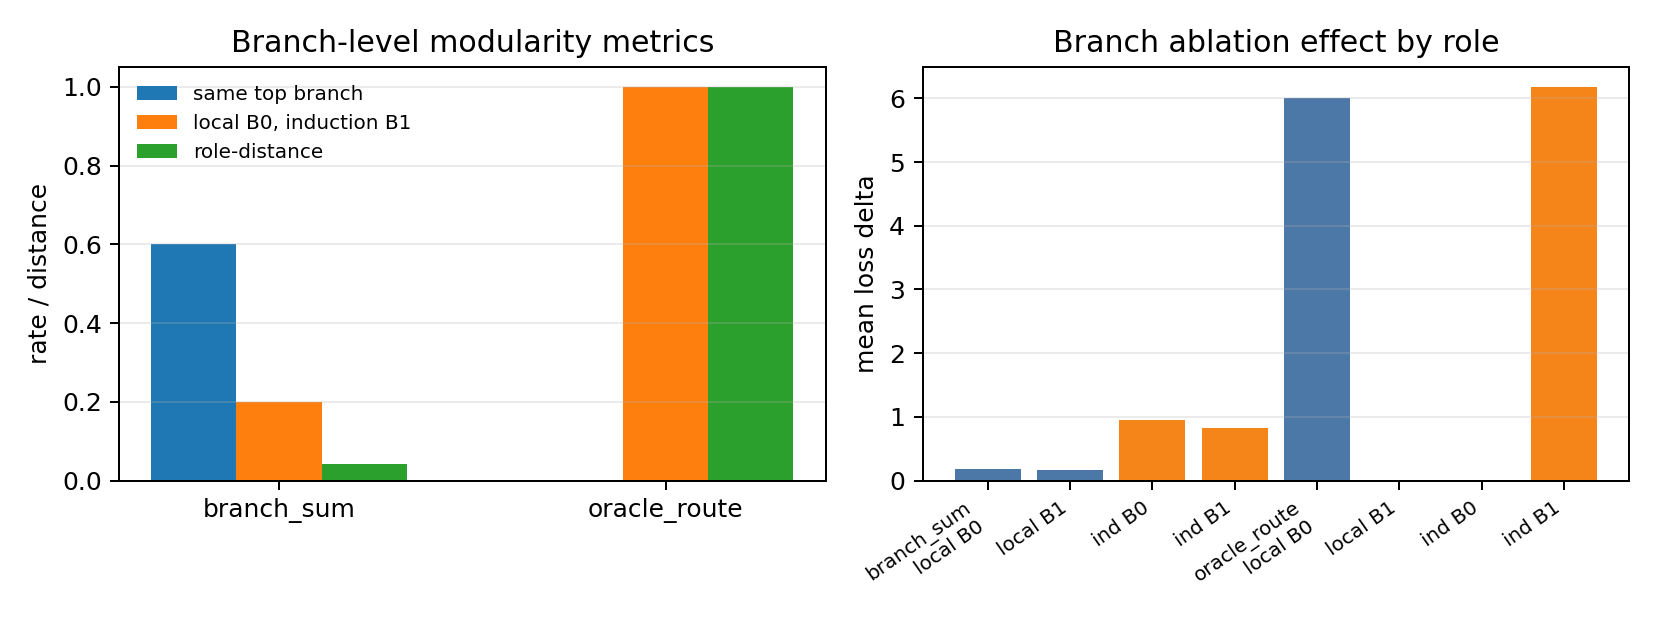
\includegraphics[width=0.9\linewidth]{figures/branch_isolation_summary.png}
  \end{center}

  \vspace{-0.4em}
  \small
  Ungated branches stay entangled. Oracle routing produces role-specific branch ablations.
\end{frame}

\begin{frame}{Summary Table}
  \begin{center}
  \scriptsize
  \begin{tabular}{lrrrrr}
    \toprule
    Config & Local acc. & Ind. acc. & Same top branch & Routed match & Branch distance \\
    \midrule
    \texttt{branch\_sum} & 1.0000 & 0.9998 & 0.60 & 0.20 & 0.0411 \\
    \texttt{oracle\_route} & 0.9999 & 0.9987 & 0.00 & 1.00 & 1.0000 \\
    \bottomrule
  \end{tabular}
  \end{center}

  \vspace{0.7em}
  Branch distance is the difference between local and induction branch-specialization
  distributions. Higher means stronger modular separation.
\end{frame}

\begin{frame}{Branch Ablation}
  \begin{center}
  \scriptsize
  \begin{tabular}{lrrrr}
    \toprule
    Config & Local B0 & Local B1 & Induction B0 & Induction B1 \\
    \midrule
    \texttt{branch\_sum} & 0.1860 & 0.1672 & 0.9538 & 0.8308 \\
    \texttt{oracle\_route} & 6.0104 & 0.0000 & 0.0000 & 6.1801 \\
    \bottomrule
  \end{tabular}
  \end{center}

  \vspace{0.7em}
  In \texttt{branch\_sum}, both branches support both roles. In
  \texttt{oracle\_route}, branch 0 is local-specific and branch 1 is
  induction-specific.
\end{frame}

\begin{frame}{Interpretation}
  \textbf{Supported:}
  \begin{itemize}
    \item Explicit routing can produce functional modularity in this toy setting.
    \item Separate branch towers alone do not discover modular roles.
    \item Specialization and modularity are experimentally separable.
  \end{itemize}

  \vspace{0.6em}
  \textbf{Current project claim:}
  \begin{quote}
    Capacity heterogeneity stabilizes specialization; routing or stronger
    structural separation is needed for robust modularity.
  \end{quote}
\end{frame}

\begin{frame}{Decision}
  Continue Phase 3 with two distinct claims:
  \begin{enumerate}
    \item structural heterogeneity can stabilize specialization;
    \item explicit routing/separation can produce modularity.
  \end{enumerate}

  \vspace{0.8em}
  Next decisive test:
  \begin{itemize}
    \item replace oracle routing with learned or weakly supervised routing;
    \item test whether modularity emerges without hard-coded task-region assignment.
  \end{itemize}
\end{frame}

\begin{frame}{Sources and Provenance}
  \scriptsize
  \begin{itemize}
    \item Report: \texttt{doc/phase3\_toy\_branch\_isolation.md}
    \item Model script: \texttt{scripts/toy\_branch\_isolation\_intervention.py}
    \item Analysis script: \texttt{scripts/analyze\_branch\_isolation.py}
    \item Run output: \texttt{results/phase3\_toy\_branch\_isolation\_lw025/}
    \item Analysis output: \texttt{results/phase3\_toy\_branch\_isolation\_analysis/}
    \item Deck data snapshot: \texttt{presentations/2026-05-22-1230-branch-isolation/data/}
  \end{itemize}
\end{frame}

\end{document}
